\newcommand{\usecase}[7]{
\begin{center}
\begin{tabular}[h!]{| l | p{12cm} |}
	\hline
	\textbf{Name} & #1 \\ \hline
	\textbf{Actors} & #2 \\ \hline
	\textbf{Goal} & #3 \\ \hline
	\textbf{Preconditions} & #4 \\ \hline
	\textbf{Basic Flow} & #5 \\ \hline
	\textbf{Alternative Flow} & #6 \\ \hline
	\textbf{Postconditions} & #7 \\ \hline
\end{tabular}
\end{center}
}

\section{Use Case Diagram}

\begin{center}
	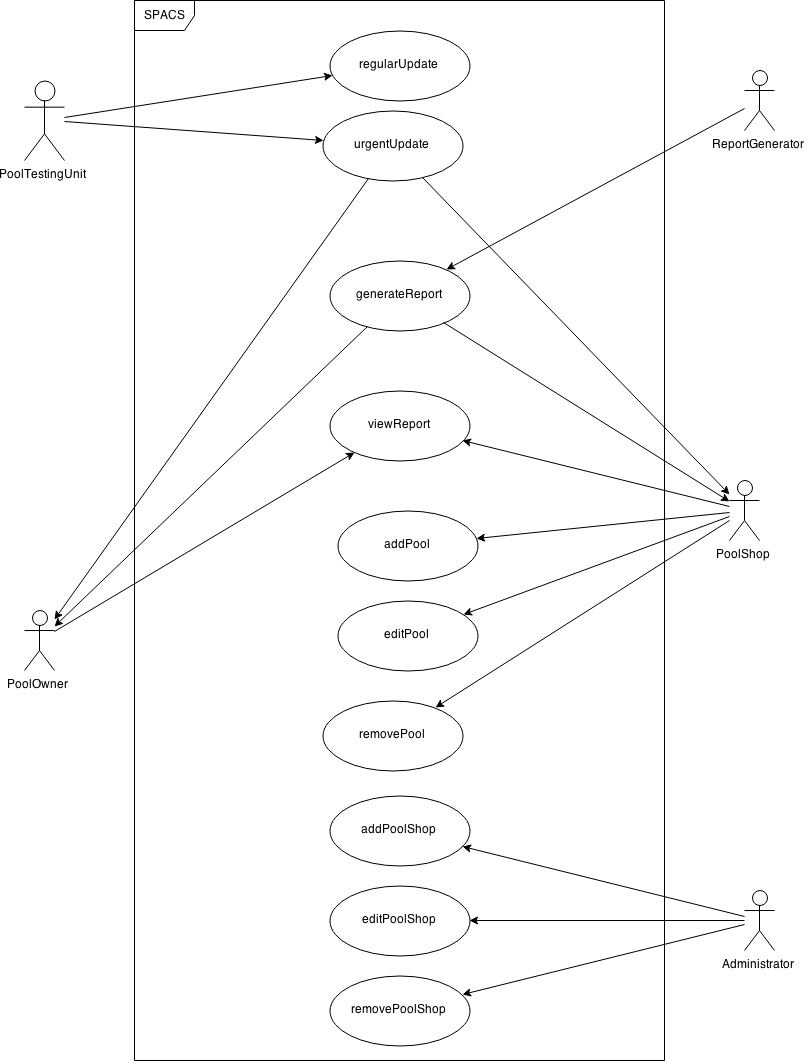
\includegraphics[width=15cm]{images/UseCaseDiagram}
\end{center}

\usecase
{regularUpdate}
{PoolTestingUnit}
{store collected information from the PTU in the system}
{PoolTestingUnit is authenticated}
{
\begin{enumerate}
\item Use case starts when ptu sends data
\item validate data
\item store it so that it can be used later
\item The use case ends
\end{enumerate}
}
{
\begin{enumerate}
\item Data is malformed
\begin{enumerate}
\item Recieved data is logged for analysis
\end{enumerate}
\item Issue storing data
\begin{enumerate}
\item Fall back to logging data and alert the administrator
\end{enumerate}
\end{enumerate}
}
{\begin{enumerate}
\item Success: Data has been stored
\item Failure: Data has been stored in a log for analysis by admin
\end{enumerate}
}

\usecase
{urgentUpdate}
{PoolTestingUnit, PoolShopAdministrator, PoolOwner}
{store collected information from the PTU in the system and alert the pool owner and pool shop that there is a problem}
{PoolTestingUnit is authenticated}
{
\begin{enumerate}
\item use case starts when ptu sends data with alerts
\item validate data
\item store it so that it can be used later
\item email is sent to the PoolShopOwner and PoolOwner
\item the use case ends
\end{enumerate}
}
{
\begin{enumerate}
\item Data is malformed
\begin{enumerate}
\item Recieved data is logged for analysis
\end{enumerate}
\item Issue storing data
\begin{enumerate}
\item Fall back to logging data and alert the administrator
\end{enumerate}
\item Email fails
\begin{enumerate}
\item Email gets retried and event is logged
\end{enumerate}
\end{enumerate}
}
{
\begin{enumerate}
\item Success: Data has been stored, email has been sent to PoolShopOwner and PoolOwner
\item Failure: Data has been stored in a log for analysis by admin
\end{enumerate}
}

\usecase
{generateReport}
{PoolOwner, PoolShopAdministrator}
{provide latest data to }
{First week of the PTU or a month since the last report}
{
\begin{enumerate}
\item use case starts at the same time every day
\item gets a list of pools that need reports
\item for each pool
\item gets the information that should be on the report
\item generates the report as a pdf
\item emails it off
\end{enumerate}
}
{}
{
\begin{enumerate}
\item Success: Report generated and emailed to pool owner and pool shop
\item Failure: Any errors logged for admin to look over
\end{enumerate}
}

\usecase
{addPoolShop}
{Administrator}
{To add a pool shop to the system.}
{}
{
\begin{enumerate}
\item Administrative user enters information about the pool shop
\end{enumerate}
}
{  - Invalid Information
    - Error displayed and user is able to re-enter}
{Success: Data is stored and can be retieved later
Failure: User is given achance to modify data}

\usecase
{editPoolShop}
{Administrator}
{To edit a pool shop in the system.}
{}
{
\begin{enumerate}
\item Administrative user enters updated information about the pool shop
\end{enumerate}
}
{
\begin{enumerate}
\item Invalid Information
\begin{enumerate}
\item Error displayed and user is able to re-enter
\end{enumerate}
\end{enumerate}
}
{
\begin{enumerate}
\item Success: Data is stored and can be retieved later
\item Failure: User is given achance to modify data
\end{enumerate}
}

\usecase
{removePoolShop}
{Administrator}
{To remove a pool shop from the system.}
{}
{
\begin{enumerate}
\item Administrative selects the pool shop
\item Confirms that the pool shop should be disabled
\end{enumerate}}
{
\begin{enumerate}
\item Cancelled
\begin{enumerate}
\item No change is made
\end{enumerate}
\end{enumerate}
}
{
\begin{enumerate}
\item Success: Data is no longer accessible. User no longer able to log in
\item Failure: No change
\end{enumerate}
}

\usecase
{addPool}
{PoolShopAdministrator}
{To add a pool to the system.}
{}
{}
{}
{}

\usecase
{editPool}
{PoolShopAdministrator}
{To edit a pool in the system.}
{}
{}
{}
{}

\usecase
{removePool}
{PoolShopAdministrator}
{To remove a pool from the system.}
{}
{}
{}
{}




